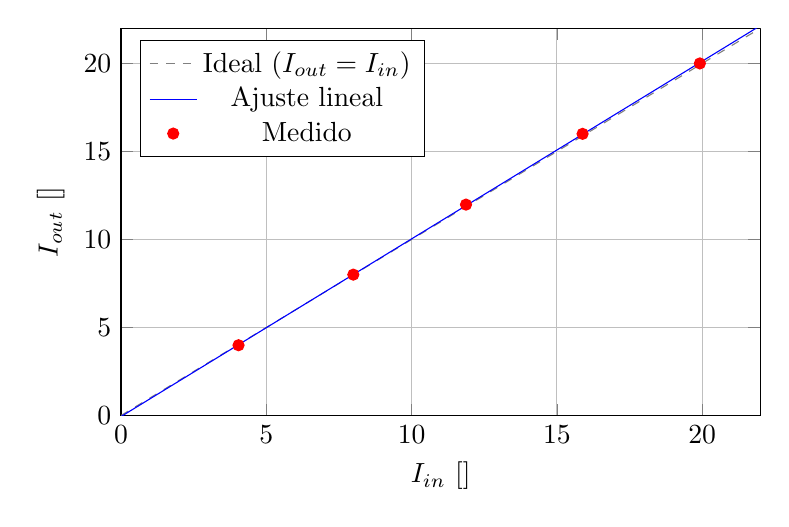
\begin{tikzpicture}
  \begin{axis}[
      width=0.8\textwidth, height=6.5cm,
      xlabel={$I_{in}$ [\si{\milli\ampere}]}, ylabel={$I_{out}$ [\si{\milli\ampere}]},
      xmin=0, xmax=22, ymin=0, ymax=22,
      grid=both, legend pos=north west,
    ]
    \addplot[gray, dashed, domain=0:22] {x};
    \addlegendentry{Ideal ($I_{out} = I_{in}$)}
    \addplot[blue, domain=0:22] {1.0093*x - 0.059};
    \addlegendentry{Ajuste lineal}
    \addplot[only marks, mark=*, red] coordinates {
      (4.044, 3.992) (7.994, 8.002) (11.872, 11.980) (15.884, 16.000) (19.920, 20.000)
    };
    \addlegendentry{Medido}
  \end{axis}
\end{tikzpicture}
